\documentclass[tikz]{standalone}

\usepackage{tikz}
\usetikzlibrary{trees}
\usetikzlibrary{shapes}
\usetikzlibrary{positioning}
\usetikzlibrary{arrows.meta}

\tikzset{
    pointer/.style = {thick,draw=black,triangle 45-*,shorten >=-3pt},
    cell/.style = {rectangle, thick, draw=black,minimum width = 1cm, minimum height =1.0cm,fill=yellow!20},
    mynode/.style = {circle, thick, draw=black, align=center,fill=yellow!40,font=\ttfamily\bfseries\Large},
    mynoder/.style = {circle, thick, draw=black, align=center,fill=red!30,font=\ttfamily\bfseries\Large},
    mynodeb/.style = {circle, thick, draw=black, align=center,fill=blue!30,font=\ttfamily\bfseries\Large},
    edgen/.style = {-latex,ultra thick},
    edger/.style = {-latex,ultra thick,red},
    edgeb/.style = {-latex,ultra thick,blue},
    edgeg/.style = {-latex,ultra thick,gray},
    edgegd/.style = {-latex,ultra thick,brown,dashed}, % back
    edgevd/.style = {-latex,ultra thick,violet,dotted}, % forward
    edgexd/.style = {-latex,ultra thick,blue,densely dotted}, % traversal
    every picture/.style={/utils/exec={\ttfamily\bfseries}},
    every picture/.style={font issue=\ttfamily\bfseries},
    font issue/.style={execute at begin picture={#1\selectfont}
  }
}

\begin{document}

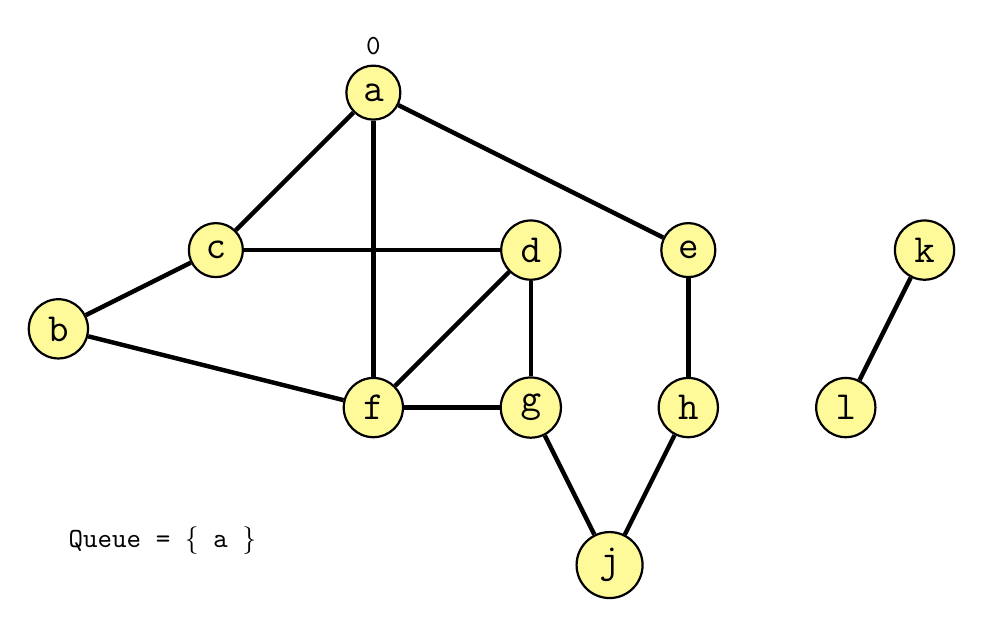
\begin{tikzpicture}[scale=1.00,transform shape]
%
\node[mynode, label={0}] at (4, 0) (a) {a};
\node[mynode] at (0,-3) (b) {b};
\node[mynode] at (2,-2) (c) {c};
\node[mynode] at (6,-2) (d) {d};
\node[mynode] at (8,-2) (e) {e};
\node[mynode] at (4,-4) (f) {f};
\node[mynode] at (6,-4) (g) {g};
\node[mynode] at (8,-4) (h) {h};
\node[mynode] at (7,-6) (j) {j};
\node[mynode] at (11,-2) (k) {k};
\node[mynode] at (10,-4) (l) {l};
\node[align=left,above right,draw=none] at (0,-6) {Queue = \{ a \}};
%
\draw[edgen,-] (a) edge node {} (c);
\draw[edgen,-] (a) edge node {} (e);
\draw[edgen,-] (a) edge node {} (f);
\draw[edgen,-] (b) edge node {} (c);
\draw[edgen,-] (b) edge node {} (f);
\draw[edgen,-] (c) edge node {} (d);
\draw[edgen,-] (f) edge node {} (g);
\draw[edgen,-] (d) edge node {} (g);
\draw[edgen,-] (e) edge node {} (h);
\draw[edgen,-] (k) edge node {} (l);
\draw[edgen,-] (f) edge node {} (d);
\draw[edgen,-] (g) edge node {} (j);
\draw[edgen,-] (h) edge node {} (j);
\end{tikzpicture}

\newpage
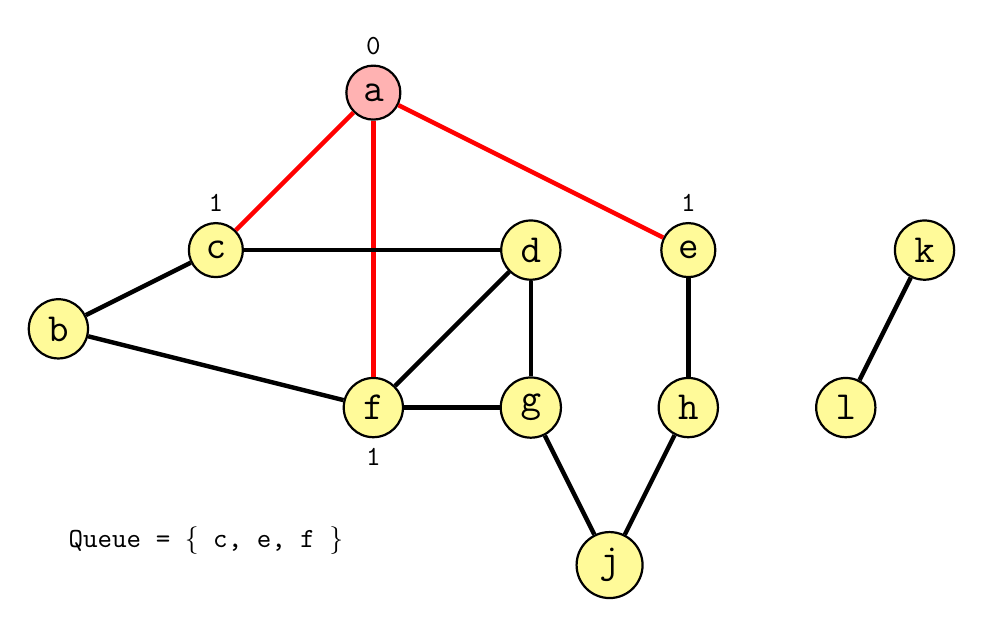
\begin{tikzpicture}[scale=1.00,transform shape]
%
\node[mynoder, label={0}] at (4, 0) (a) {a};
\node[mynode] at (0,-3) (b) {b};
\node[mynode, label={1}] at (2,-2) (c) {c};
\node[mynode] at (6,-2) (d) {d};
\node[mynode, label={1}] at (8,-2) (e) {e};
\node[mynode, label={below:1}] at (4,-4) (f) {f};
\node[mynode] at (6,-4) (g) {g};
\node[mynode] at (8,-4) (h) {h};
\node[mynode] at (7,-6) (j) {j};
\node[mynode] at (11,-2) (k) {k};
\node[mynode] at (10,-4) (l) {l};
\node[align=left,above right,draw=none] at (0,-6) {Queue = \{ c, e, f \}};
%
\draw[edger,-] (a) edge node {} (c);
\draw[edger,-] (a) edge node {} (e);
\draw[edger,-] (a) edge node {} (f);
\draw[edgen,-] (b) edge node {} (c);
\draw[edgen,-] (b) edge node {} (f);
\draw[edgen,-] (c) edge node {} (d);
\draw[edgen,-] (f) edge node {} (g);
\draw[edgen,-] (d) edge node {} (g);
\draw[edgen,-] (e) edge node {} (h);
\draw[edgen,-] (k) edge node {} (l);
\draw[edgen,-] (f) edge node {} (d);
\draw[edgen,-] (g) edge node {} (j);
\draw[edgen,-] (h) edge node {} (j);
\end{tikzpicture}

\newpage
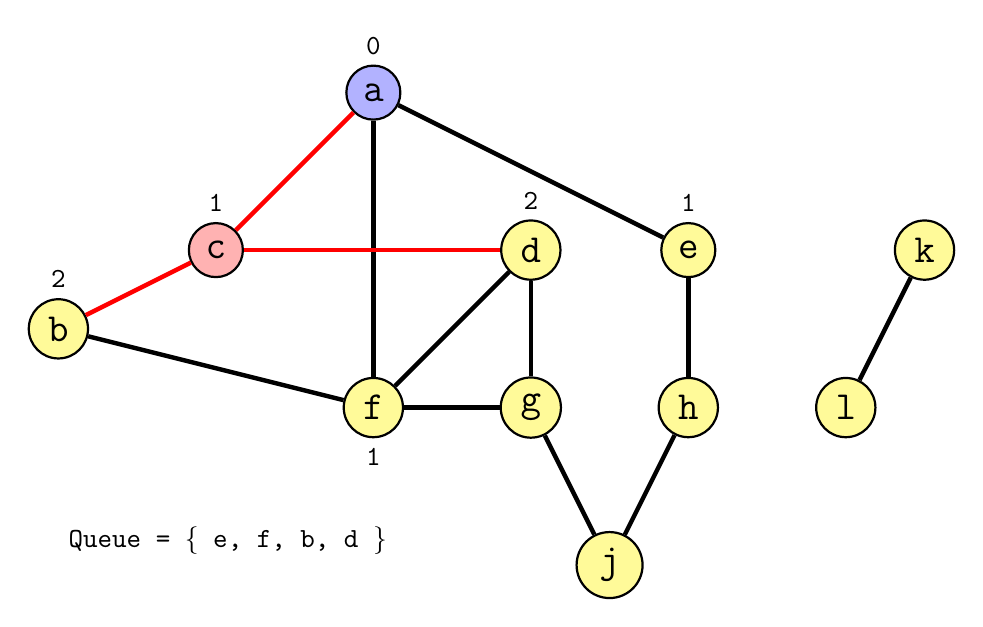
\begin{tikzpicture}[scale=1.00,transform shape]
%
\node[mynodeb, label={0}] at (4, 0) (a) {a};
\node[mynode, label={2}] at (0,-3) (b) {b};
\node[mynoder, label={1}] at (2,-2) (c) {c};
\node[mynode, label={2}] at (6,-2) (d) {d};
\node[mynode, label={1}] at (8,-2) (e) {e};
\node[mynode, label={below:1}] at (4,-4) (f) {f};
\node[mynode] at (6,-4) (g) {g};
\node[mynode] at (8,-4) (h) {h};
\node[mynode] at (7,-6) (j) {j};
\node[mynode] at (11,-2) (k) {k};
\node[mynode] at (10,-4) (l) {l};
\node[align=left,above right,draw=none] at (0,-6) {Queue = \{ e, f, b, d \}};
%
\draw[edger,-] (a) edge node {} (c);
\draw[edgen,-] (a) edge node {} (e);
\draw[edgen,-] (a) edge node {} (f);
\draw[edger,-] (b) edge node {} (c);
\draw[edgen,-] (b) edge node {} (f);
\draw[edger,-] (c) edge node {} (d);
\draw[edgen,-] (f) edge node {} (g);
\draw[edgen,-] (d) edge node {} (g);
\draw[edgen,-] (e) edge node {} (h);
\draw[edgen,-] (k) edge node {} (l);
\draw[edgen,-] (f) edge node {} (d);
\draw[edgen,-] (g) edge node {} (j);
\draw[edgen,-] (h) edge node {} (j);
\end{tikzpicture}

\newpage
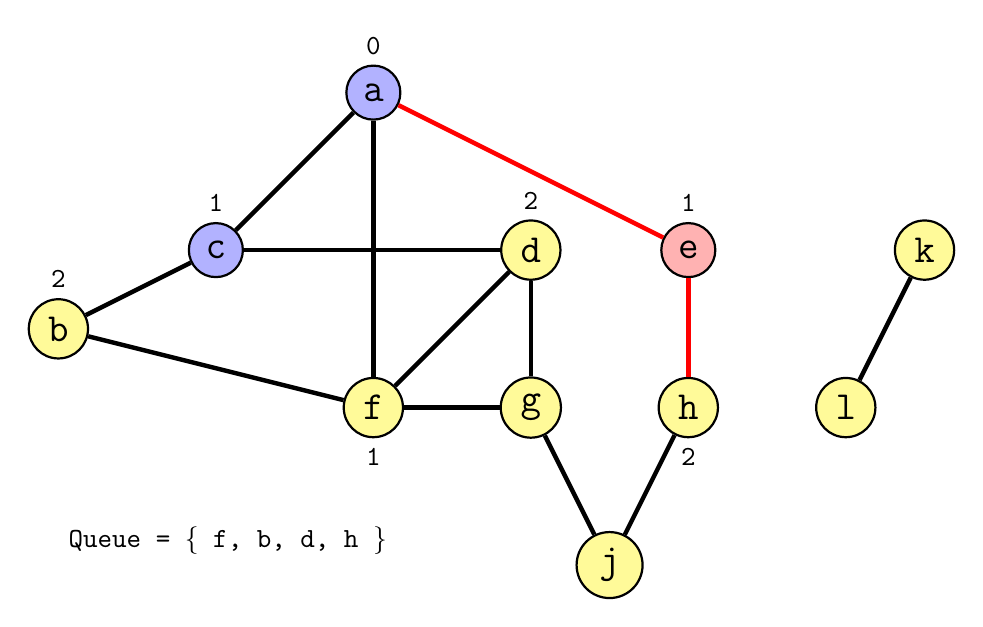
\begin{tikzpicture}[scale=1.00,transform shape]
%
\node[mynodeb, label={0}] at (4, 0) (a) {a};
\node[mynode, label={2}] at (0,-3) (b) {b};
\node[mynodeb, label={1}] at (2,-2) (c) {c};
\node[mynode, label={2}] at (6,-2) (d) {d};
\node[mynoder, label={1}] at (8,-2) (e) {e};
\node[mynode, label={below:1}] at (4,-4) (f) {f};
\node[mynode] at (6,-4) (g) {g};
\node[mynode, label={below:2}] at (8,-4) (h) {h};
\node[mynode] at (7,-6) (j) {j};
\node[mynode] at (11,-2) (k) {k};
\node[mynode] at (10,-4) (l) {l};
\node[align=left,above right,draw=none] at (0,-6) {Queue = \{ f, b, d, h \}};
%
\draw[edgen,-] (a) edge node {} (c);
\draw[edger,-] (a) edge node {} (e);
\draw[edgen,-] (a) edge node {} (f);
\draw[edgen,-] (b) edge node {} (c);
\draw[edgen,-] (b) edge node {} (f);
\draw[edgen,-] (c) edge node {} (d);
\draw[edgen,-] (f) edge node {} (g);
\draw[edgen,-] (d) edge node {} (g);
\draw[edger,-] (e) edge node {} (h);
\draw[edgen,-] (k) edge node {} (l);
\draw[edgen,-] (f) edge node {} (d);
\draw[edgen,-] (g) edge node {} (j);
\draw[edgen,-] (h) edge node {} (j);
\end{tikzpicture}

\newpage
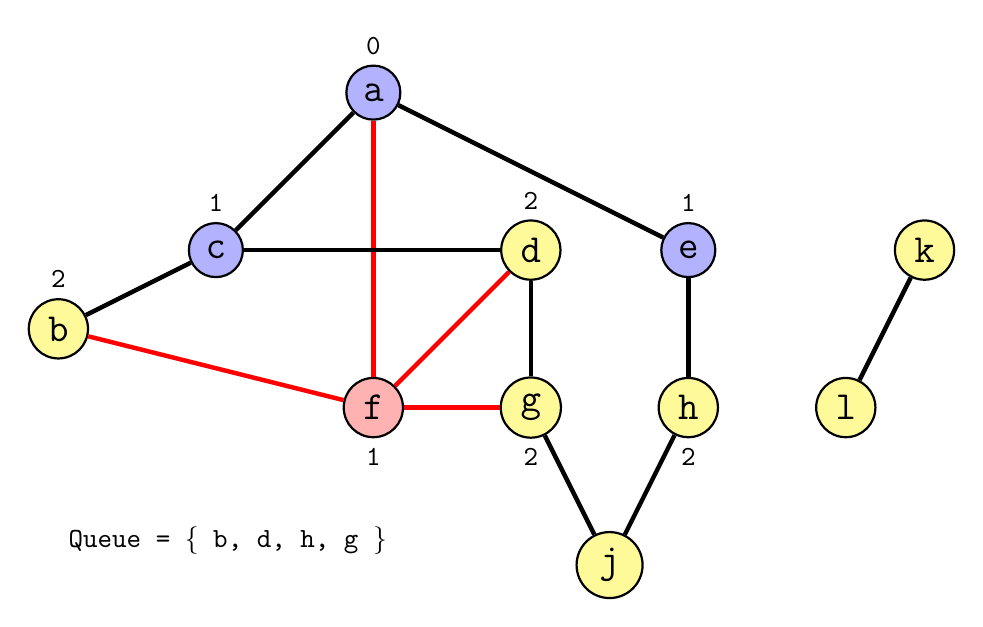
\begin{tikzpicture}[scale=1.00,transform shape]
%
\node[mynodeb, label={0}] at (4, 0) (a) {a};
\node[mynode, label={2}] at (0,-3) (b) {b};
\node[mynodeb, label={1}] at (2,-2) (c) {c};
\node[mynode, label={2}] at (6,-2) (d) {d};
\node[mynodeb, label={1}] at (8,-2) (e) {e};
\node[mynoder, label={below:1}] at (4,-4) (f) {f};
\node[mynode, label={below:2}] at (6,-4) (g) {g};
\node[mynode, label={below:2}] at (8,-4) (h) {h};
\node[mynode] at (7,-6) (j) {j};
\node[mynode] at (11,-2) (k) {k};
\node[mynode] at (10,-4) (l) {l};
\node[align=left,above right,draw=none] at (0,-6) {Queue = \{ b, d, h, g \}};
%
\draw[edgen,-] (a) edge node {} (c);
\draw[edgen,-] (a) edge node {} (e);
\draw[edger,-] (a) edge node {} (f);
\draw[edgen,-] (b) edge node {} (c);
\draw[edger,-] (b) edge node {} (f);
\draw[edgen,-] (c) edge node {} (d);
\draw[edger,-] (f) edge node {} (g);
\draw[edgen,-] (d) edge node {} (g);
\draw[edgen,-] (e) edge node {} (h);
\draw[edgen,-] (k) edge node {} (l);
\draw[edger,-] (f) edge node {} (d);
\draw[edgen,-] (g) edge node {} (j);
\draw[edgen,-] (h) edge node {} (j);
\end{tikzpicture}

\newpage
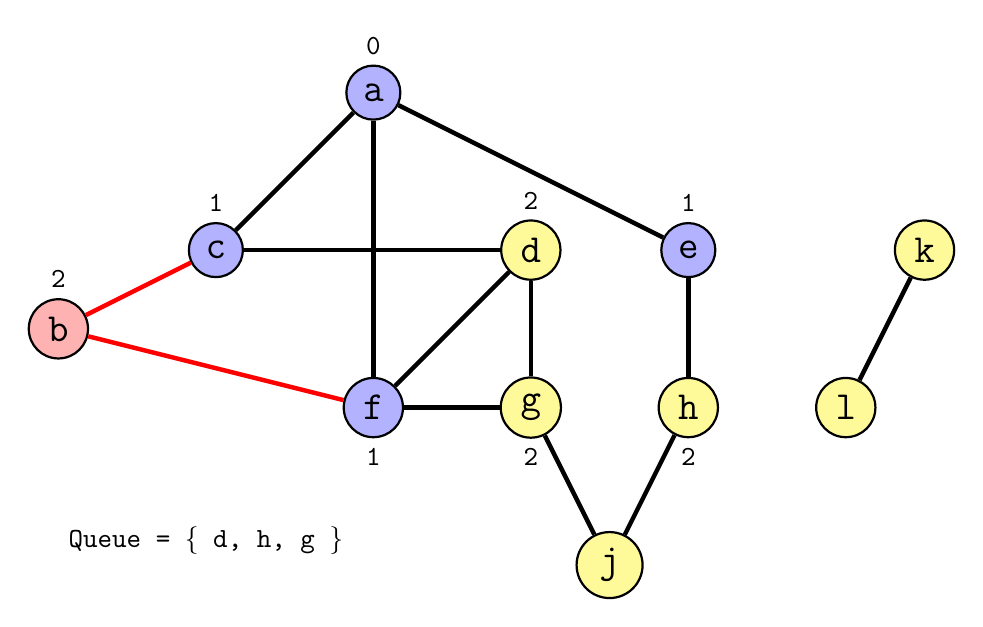
\begin{tikzpicture}[scale=1.00,transform shape]
%
\node[mynodeb, label={0}] at (4, 0) (a) {a};
\node[mynoder, label={2}] at (0,-3) (b) {b};
\node[mynodeb, label={1}] at (2,-2) (c) {c};
\node[mynode, label={2}] at (6,-2) (d) {d};
\node[mynodeb, label={1}] at (8,-2) (e) {e};
\node[mynodeb, label={below:1}] at (4,-4) (f) {f};
\node[mynode, label={below:2}] at (6,-4) (g) {g};
\node[mynode, label={below:2}] at (8,-4) (h) {h};
\node[mynode] at (7,-6) (j) {j};
\node[mynode] at (11,-2) (k) {k};
\node[mynode] at (10,-4) (l) {l};
\node[align=left,above right,draw=none] at (0,-6) {Queue = \{ d, h, g \}};
%
\draw[edgen,-] (a) edge node {} (c);
\draw[edgen,-] (a) edge node {} (e);
\draw[edgen,-] (a) edge node {} (f);
\draw[edger,-] (b) edge node {} (c);
\draw[edger,-] (b) edge node {} (f);
\draw[edgen,-] (c) edge node {} (d);
\draw[edgen,-] (f) edge node {} (g);
\draw[edgen,-] (d) edge node {} (g);
\draw[edgen,-] (e) edge node {} (h);
\draw[edgen,-] (k) edge node {} (l);
\draw[edgen,-] (f) edge node {} (d);
\draw[edgen,-] (g) edge node {} (j);
\draw[edgen,-] (h) edge node {} (j);
\end{tikzpicture}

\newpage
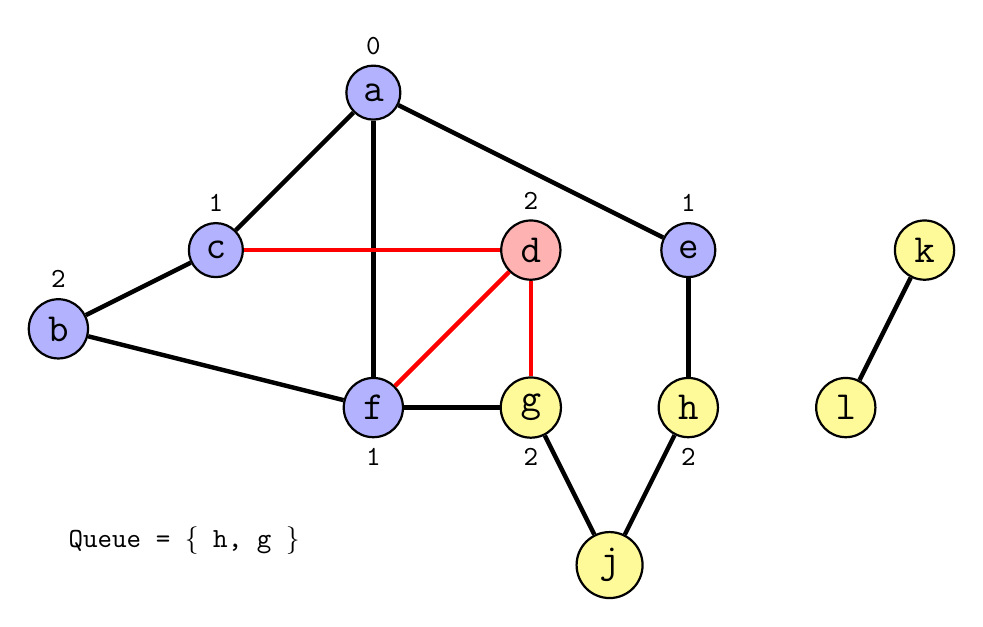
\begin{tikzpicture}[scale=1.00,transform shape]
%
\node[mynodeb, label={0}] at (4, 0) (a) {a};
\node[mynodeb, label={2}] at (0,-3) (b) {b};
\node[mynodeb, label={1}] at (2,-2) (c) {c};
\node[mynoder, label={2}] at (6,-2) (d) {d};
\node[mynodeb, label={1}] at (8,-2) (e) {e};
\node[mynodeb, label={below:1}] at (4,-4) (f) {f};
\node[mynode, label={below:2}] at (6,-4) (g) {g};
\node[mynode, label={below:2}] at (8,-4) (h) {h};
\node[mynode] at (7,-6) (j) {j};
\node[mynode] at (11,-2) (k) {k};
\node[mynode] at (10,-4) (l) {l};
\node[align=left,above right,draw=none] at (0,-6) {Queue = \{ h, g \}};
%
\draw[edgen,-] (a) edge node {} (c);
\draw[edgen,-] (a) edge node {} (e);
\draw[edgen,-] (a) edge node {} (f);
\draw[edgen,-] (b) edge node {} (c);
\draw[edgen,-] (b) edge node {} (f);
\draw[edger,-] (c) edge node {} (d);
\draw[edgen,-] (f) edge node {} (g);
\draw[edger,-] (d) edge node {} (g);
\draw[edgen,-] (e) edge node {} (h);
\draw[edgen,-] (k) edge node {} (l);
\draw[edger,-] (f) edge node {} (d);
\draw[edgen,-] (g) edge node {} (j);
\draw[edgen,-] (h) edge node {} (j);
\end{tikzpicture}

\newpage
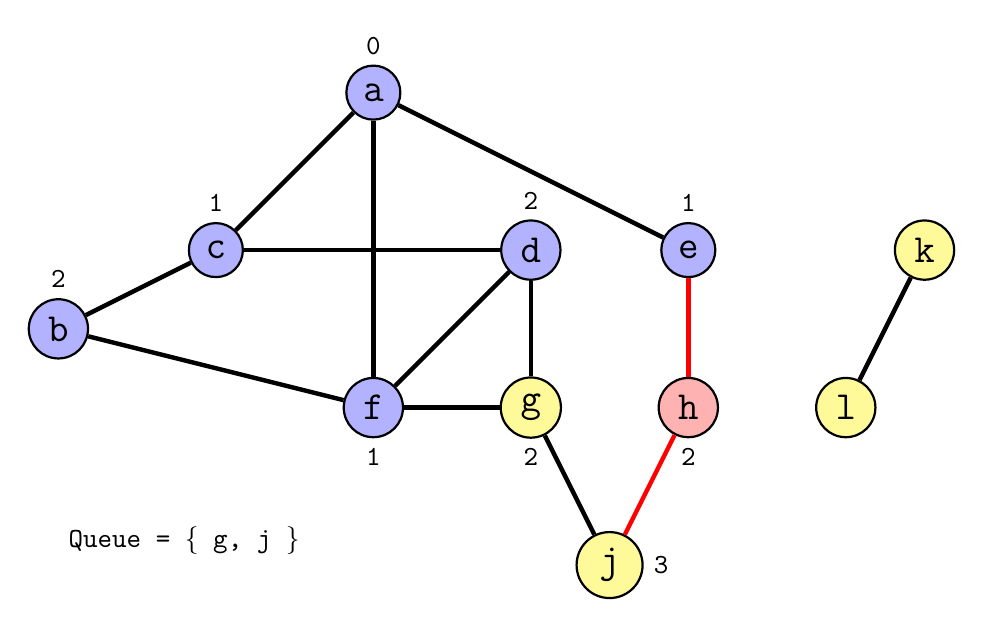
\begin{tikzpicture}[scale=1.00,transform shape]
%
\node[mynodeb, label={0}] at (4, 0) (a) {a};
\node[mynodeb, label={2}] at (0,-3) (b) {b};
\node[mynodeb, label={1}] at (2,-2) (c) {c};
\node[mynodeb, label={2}] at (6,-2) (d) {d};
\node[mynodeb, label={1}] at (8,-2) (e) {e};
\node[mynodeb, label={below:1}] at (4,-4) (f) {f};
\node[mynode, label={below:2}] at (6,-4) (g) {g};
\node[mynoder, label={below:2}] at (8,-4) (h) {h};
\node[mynode, label={right:3}] at (7,-6) (j) {j};
\node[mynode] at (11,-2) (k) {k};
\node[mynode] at (10,-4) (l) {l};
\node[align=left,above right,draw=none] at (0,-6) {Queue = \{ g, j \}};
%
\draw[edgen,-] (a) edge node {} (c);
\draw[edgen,-] (a) edge node {} (e);
\draw[edgen,-] (a) edge node {} (f);
\draw[edgen,-] (b) edge node {} (c);
\draw[edgen,-] (b) edge node {} (f);
\draw[edgen,-] (c) edge node {} (d);
\draw[edgen,-] (f) edge node {} (g);
\draw[edgen,-] (d) edge node {} (g);
\draw[edger,-] (e) edge node {} (h);
\draw[edgen,-] (k) edge node {} (l);
\draw[edgen,-] (f) edge node {} (d);
\draw[edgen,-] (g) edge node {} (j);
\draw[edger,-] (h) edge node {} (j);
\end{tikzpicture}

\newpage
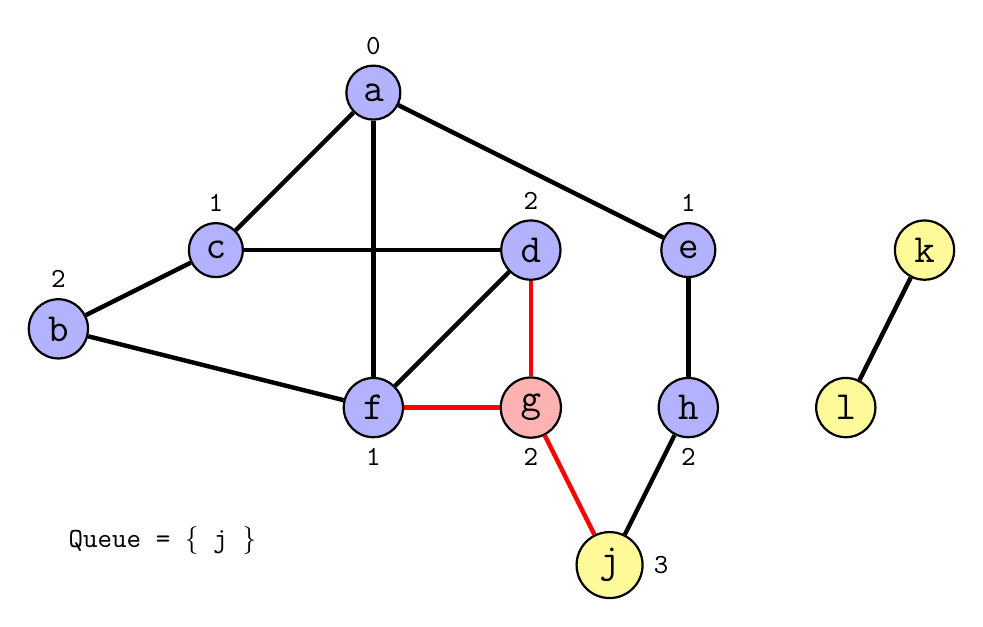
\begin{tikzpicture}[scale=1.00,transform shape]
%
\node[mynodeb, label={0}] at (4, 0) (a) {a};
\node[mynodeb, label={2}] at (0,-3) (b) {b};
\node[mynodeb, label={1}] at (2,-2) (c) {c};
\node[mynodeb, label={2}] at (6,-2) (d) {d};
\node[mynodeb, label={1}] at (8,-2) (e) {e};
\node[mynodeb, label={below:1}] at (4,-4) (f) {f};
\node[mynoder, label={below:2}] at (6,-4) (g) {g};
\node[mynodeb, label={below:2}] at (8,-4) (h) {h};
\node[mynode, label={right:3}] at (7,-6) (j) {j};
\node[mynode] at (11,-2) (k) {k};
\node[mynode] at (10,-4) (l) {l};
\node[align=left,above right,draw=none] at (0,-6) {Queue = \{ j \}};
%
\draw[edgen,-] (a) edge node {} (c);
\draw[edgen,-] (a) edge node {} (e);
\draw[edgen,-] (a) edge node {} (f);
\draw[edgen,-] (b) edge node {} (c);
\draw[edgen,-] (b) edge node {} (f);
\draw[edgen,-] (c) edge node {} (d);
\draw[edger,-] (f) edge node {} (g);
\draw[edger,-] (d) edge node {} (g);
\draw[edgen,-] (e) edge node {} (h);
\draw[edgen,-] (k) edge node {} (l);
\draw[edgen,-] (f) edge node {} (d);
\draw[edger,-] (g) edge node {} (j);
\draw[edgen,-] (h) edge node {} (j);
\end{tikzpicture}

\newpage
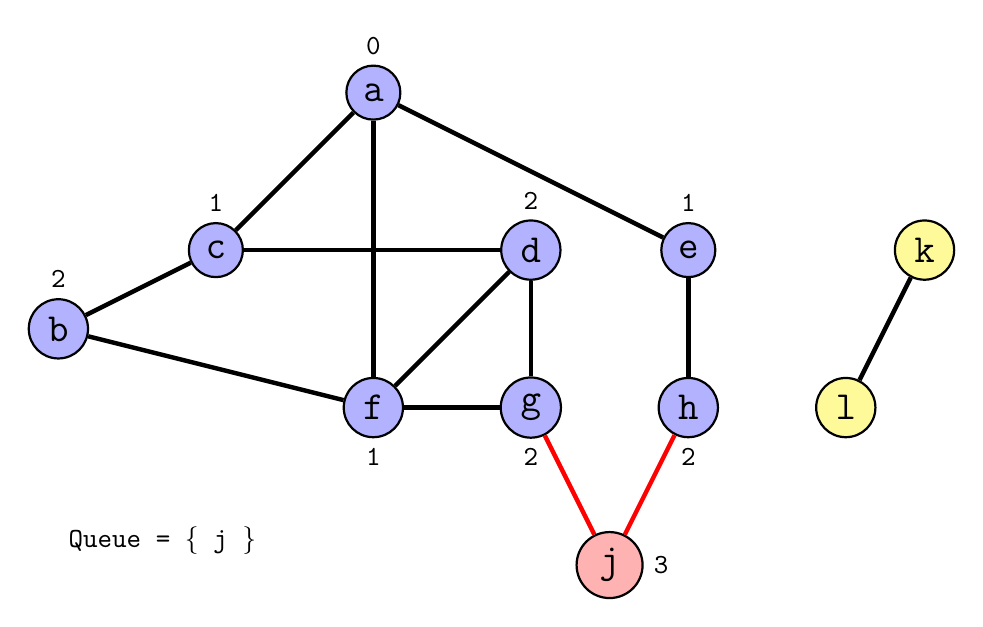
\begin{tikzpicture}[scale=1.00,transform shape]
%
\node[mynodeb, label={0}] at (4, 0) (a) {a};
\node[mynodeb, label={2}] at (0,-3) (b) {b};
\node[mynodeb, label={1}] at (2,-2) (c) {c};
\node[mynodeb, label={2}] at (6,-2) (d) {d};
\node[mynodeb, label={1}] at (8,-2) (e) {e};
\node[mynodeb, label={below:1}] at (4,-4) (f) {f};
\node[mynodeb, label={below:2}] at (6,-4) (g) {g};
\node[mynodeb, label={below:2}] at (8,-4) (h) {h};
\node[mynoder, label={right:3}] at (7,-6) (j) {j};
\node[mynode] at (11,-2) (k) {k};
\node[mynode] at (10,-4) (l) {l};
\node[align=left,above right,draw=none] at (0,-6) {Queue = \{ j \}};
%
\draw[edgen,-] (a) edge node {} (c);
\draw[edgen,-] (a) edge node {} (e);
\draw[edgen,-] (a) edge node {} (f);
\draw[edgen,-] (b) edge node {} (c);
\draw[edgen,-] (b) edge node {} (f);
\draw[edgen,-] (c) edge node {} (d);
\draw[edgen,-] (f) edge node {} (g);
\draw[edgen,-] (d) edge node {} (g);
\draw[edgen,-] (e) edge node {} (h);
\draw[edgen,-] (k) edge node {} (l);
\draw[edgen,-] (f) edge node {} (d);
\draw[edger,-] (g) edge node {} (j);
\draw[edger,-] (h) edge node {} (j);
\end{tikzpicture}

\newpage
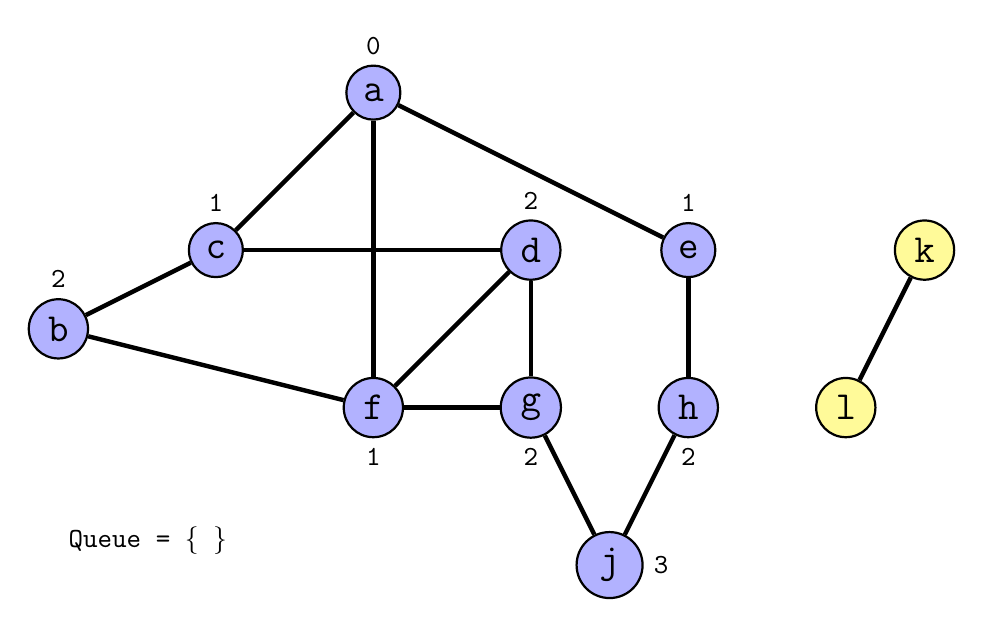
\begin{tikzpicture}[scale=1.00,transform shape]
%
\node[mynodeb, label={0}] at (4, 0) (a) {a};
\node[mynodeb, label={2}] at (0,-3) (b) {b};
\node[mynodeb, label={1}] at (2,-2) (c) {c};
\node[mynodeb, label={2}] at (6,-2) (d) {d};
\node[mynodeb, label={1}] at (8,-2) (e) {e};
\node[mynodeb, label={below:1}] at (4,-4) (f) {f};
\node[mynodeb, label={below:2}] at (6,-4) (g) {g};
\node[mynodeb, label={below:2}] at (8,-4) (h) {h};
\node[mynodeb, label={right:3}] at (7,-6) (j) {j};
\node[mynode] at (11,-2) (k) {k};
\node[mynode] at (10,-4) (l) {l};
\node[align=left,above right,draw=none] at (0,-6) {Queue = \{ \}};
%
\draw[edgen,-] (a) edge node {} (c);
\draw[edgen,-] (a) edge node {} (e);
\draw[edgen,-] (a) edge node {} (f);
\draw[edgen,-] (b) edge node {} (c);
\draw[edgen,-] (b) edge node {} (f);
\draw[edgen,-] (c) edge node {} (d);
\draw[edgen,-] (f) edge node {} (g);
\draw[edgen,-] (d) edge node {} (g);
\draw[edgen,-] (e) edge node {} (h);
\draw[edgen,-] (k) edge node {} (l);
\draw[edgen,-] (f) edge node {} (d);
\draw[edgen,-] (g) edge node {} (j);
\draw[edgen,-] (h) edge node {} (j);
\end{tikzpicture}

\newpage
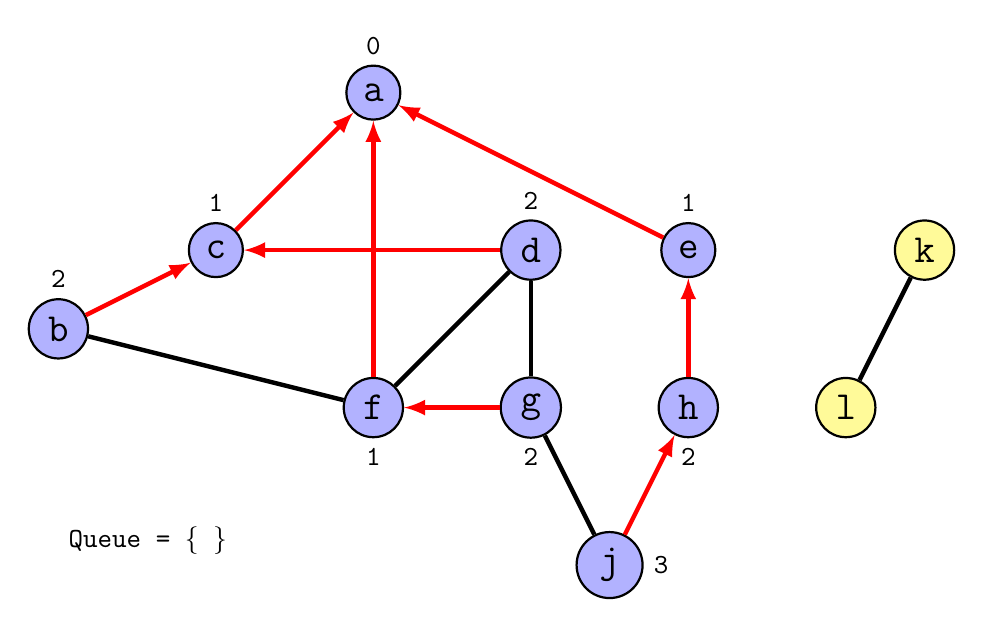
\begin{tikzpicture}[scale=1.00,transform shape]
%
\node[mynodeb, label={0}] at (4, 0) (a) {a};
\node[mynodeb, label={2}] at (0,-3) (b) {b};
\node[mynodeb, label={1}] at (2,-2) (c) {c};
\node[mynodeb, label={2}] at (6,-2) (d) {d};
\node[mynodeb, label={1}] at (8,-2) (e) {e};
\node[mynodeb, label={below:1}] at (4,-4) (f) {f};
\node[mynodeb, label={below:2}] at (6,-4) (g) {g};
\node[mynodeb, label={below:2}] at (8,-4) (h) {h};
\node[mynodeb, label={right:3}] at (7,-6) (j) {j};
\node[mynode] at (11,-2) (k) {k};
\node[mynode] at (10,-4) (l) {l};
\node[align=left,above right,draw=none] at (0,-6) {Queue = \{ \}};
%
\draw[edger] (c) edge node {} (a);
\draw[edger] (e) edge node {} (a);
\draw[edger] (f) edge node {} (a);
\draw[edger] (b) edge node {} (c);
\draw[edger] (d) edge node {} (c);
\draw[edger] (h) edge node {} (e);
\draw[edger] (j) edge node {} (h);
\draw[edgen,-] (g) edge node {} (d);
\draw[edgen,-] (b) edge node {} (f);
\draw[edger] (g) edge node {} (f);
\draw[edgen,-] (k) edge node {} (l);
\draw[edgen,-] (f) edge node {} (d);
\draw[edgen,-] (g) edge node {} (j);
\end{tikzpicture}

\end{document}